\newpage
\solutions{Szachownice, klocki i kolorowanie}

\begin{problem}{1}
	Szachownicę o wymiarach $15 \times 15$ przykryto przy pomocy płytek o wymiarach $2 \times 2$ i $3 \times 3$ w taki sposób, że każde pole jest przykryte przez dokładnie jedną płytką oraz płytki nie wystają poza szachownicę. Wyznaczyć najmniejszą liczbę użytych płytek $3 \times 3$, dla której jest to możliwe.
\end{problem}

\answer{Minimalną liczbą płytek $3 \times 3$, dla których istnieje szukane pokrycie planszy jest $9$.}

\noindent
Pokrycie planszy za pomocą $9$ klocków jest zobrazowane na poniższej ilustarcji.

\begin{center}
	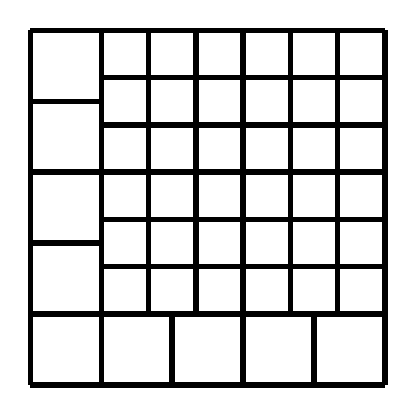
\begin{tikzpicture}[scale=0.3]


		\draw[line width=2pt] (0,0) -- (15,0);
		\draw[line width=2pt] (0,3) -- (15,3);
		\draw[line width=2pt] (3,0) -- (3,15);
		\draw[line width=2pt] (0,0) -- (0,15);
		\draw[line width=2pt] (0,15) -- (3,15);
		\draw[line width=2pt] (15,0) -- (15,3);

		\draw[line width=2pt] (6,0) -- (6,3);
		\draw[line width=2pt] (9,0) -- (9,3);
		\draw[line width=2pt] (12,0) -- (12,3);

		\draw[line width=2pt] (0,6) -- (3,6);
		\draw[line width=2pt] (0,9) -- (3,9);
		\draw[line width=2pt] (0,12) -- (3,12);

		\draw[line width=2pt] (3,5) -- (15,5);
		\draw[line width=2pt] (3,7) -- (15,7);
		\draw[line width=2pt] (3,9) -- (15,9);
		\draw[line width=2pt] (3,11) -- (15,11);
		\draw[line width=2pt] (3,13) -- (15,13);
		\draw[line width=2pt] (3,15) -- (15,15);


		\draw[line width=2pt] (5,3) -- (5,15);
		\draw[line width=2pt] (7,3) -- (7,15);
		\draw[line width=2pt] (9,3) -- (9,15);
		\draw[line width=2pt] (11,3) -- (11,15);
		\draw[line width=2pt] (13,3) -- (13,15);
		\draw[line width=2pt] (15,3) -- (15,15);
	\end{tikzpicture}
\end{center}

\noindent
Załóżmy nie wprost, że istnieje szukane pokrycie, w którym użyto nie więcej niż $8$ klocków $3 \times 3$.
Zauważmy, że pól na planszy jest $15^2 = 225$. Oznaczmy liczbę płytek $2 \times 2$ jako $a$, a liczbę płytek $3 \times 3$ jako $b$. Wówczas zachodzi równość
\[
	4a + 9b = 225 \implies 4a = 225 - 9b.
\]
Jedynymi liczbami $0 \leqslant b \leqslant 8$, dla których liczba $225 - 9b$ jest podzielna przez $4$ są $b = 1$ i $b = 5$.

\vspace{10px}
\noindent
W każdym wierszu znajduje się $15$ pól. Rozpatrzmy jeden z nich. Klocek $2 \times 2$ zajmuje $0$ lub $2$ pola w tym wierszu. Skoro $15$ jest liczbą nieparzystą, to w tym wierszu znajduje się co najmniej $1$ klocek $3 \times 3$. 

\vspace{10px}
\noindent
Każdy klocek $3 \times 3$ pokrywa pola w $3$ kolejnych wierszach, których jest $15$. Jak pokazaliśmy wyżej, każdy z tych wierszy zawiera pole przykryte przez jeden z tych klocków. Wiemy również, że liczba tych klocków wynosi $1$ lub $5$. Gdy jest jeden taki klocek, to łatwo otrzymujemy sprzeczność. Gdy jest ich $5$, to leżą w wierszach $1-3$, $4-6$, $7-9$, $10-12$ i $13-15$.


\begin{center}
	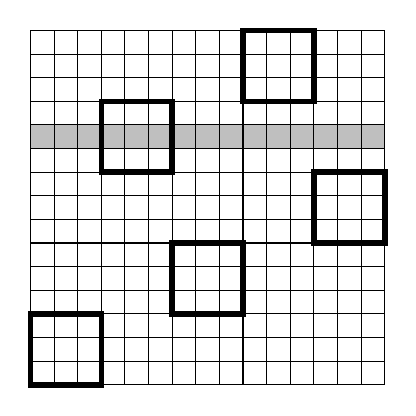
\begin{tikzpicture}[scale=0.3]

		\fill[color=gray!50] (0,10) -- (15,10) -- (15,11) -- (0,11);

		\draw (0,0) -- (15,0) -- (15,15) -- (0,15) -- cycle;
		\draw (0,1) -- (15,1);
		\draw (0,2) -- (15,2);
		\draw (0,3) -- (15,3);
		\draw (0,4) -- (15,4);
		\draw (0,5) -- (15,5);
		\draw (0,6) -- (15,6);
		\draw (0,7) -- (15,7);
		\draw (0,8) -- (15,8);
		\draw (0,9) -- (15,9);
		\draw (0,10) -- (15,10);
		\draw (0,11) -- (15,11);
		\draw (0,12) -- (15,12);
		\draw (0,13) -- (15,13);
		\draw (0,14) -- (15,14);


		\draw (1,0) -- (1,15);
		\draw (2,0) -- (2,15);
		\draw (3,0) -- (3,15);
		\draw (4,0) -- (4,15);
		\draw (5,0) -- (5,15);
		\draw (6,0) -- (6,15);
		\draw (7,0) -- (7,15);
		\draw (8,0) -- (8,15);
		\draw (9,0) -- (9,15);
		\draw (10,0) -- (10,15);
		\draw (11,0) -- (11,15);
		\draw (12,0) -- (12,15);
		\draw (13,0) -- (13,15);
		\draw (14,0) -- (14,15);

		\draw[line width=2pt] (0,0) -- (0,3) -- (3,3) -- (3,0) -- cycle;
		\draw[line width=2pt] (3,9) -- (3,12) -- (6,12) -- (6,9) -- cycle;
		\draw[line width=2pt] (6,3) -- (6,6) -- (9,6) -- (9,3) -- cycle;
		\draw[line width=2pt] (9,12) -- (9,15) -- (12,15) -- (12,12) -- cycle;
		\draw[line width=2pt] (12,6) -- (12,9) -- (15,9) -- (15,6) -- cycle;


	\end{tikzpicture}
\end{center}


\vspace{10px}
\noindent
Rozpatrzmy klocek, który leży w wierszach 4-6. Dzieli on każdy z nich na część o wysokości $3$ klocków i część o wysokości $9$ klocków. Żadnej z tych części nie da się pokryć za pomocą klocków $2 \times 2$, a wiemy, że żaden inny klocek $3 \times 3$ nie leży w tym wierszu. Otrzymujemy sprzeczność, która dowodzi, że tych klocków jest co najmniej $10$.

\vspace{5px}

\begin{problem}{2}
	Płaszczyznę pokolorowano trzema kolorami. Wykazać, że istnieje odcinek o długości $1$, który ma końce tego samego koloru.
\end{problem}

\noindent
Załóżmy nie wprost, że każdy odcinek ma końce różnych kolorów. Oznaczmy te kolory numerami $1$, $2$ i $3$. Załóżmy bez straty ogólności, że istnieje pewien punkt $X$ koloru $1$.

\vspace{10px}
\noindent
Rozpatrzmy takie punkty $A$, $B$, że trójkąt $XAB$ jest trójkątem równobocznym o boku długości $1$. Na mocy założenia ten trójkąt ma wierzchołki różnych kolorów, czyli $A$ i~$B$ mają odpowiednio kolory $3$ i $2$ lub $2$ i $3$. Weźmy taki punkt~$B'$, różny od $X$, że trójkąt~$X'AB$ jest równoboczny. Mamy wtedy, że punkt~$X'$ musi mieć różny kolor od punktów~$A$ i~$B$, czyli jest koloru $1$.

\begin{center}
	\begin{tikzpicture}[scale=0.5]
		\tkzDefPoint(0,0){A}
		\tkzDefPoint(0,2){B}
		\tkzDefEquilateral(A,B)\tkzGetPoint{X};
		\tkzDefEquilateral(B,A)\tkzGetPoint{X'};

		\tkzDrawPoints(A,B,X,X');
		\tkzDrawSegments(A,B A,X B,X A,X' B,X');
		\tkzDrawCircle[dashed](X,X');

		\tkzLabelPoint[left](X){$A$}
		\tkzLabelPoint[right](X'){$X'$}
		\tkzLabelPoint[below](A){$A$}
		\tkzLabelPoint[above](B){$B$}
	\end{tikzpicture}
\end{center}

\noindent
Analogicznie można wykazać, że każdy punkt oddalony od $X$ o długość odcinka $XX'$ jest koloru $1$. Biorąc dwa punkty, oddalone o $1$, leżące na okręgu o środku w $X$ i promieniu $XX'$, otrzymujemy sprzeczność.


\begin{problem}{3}
	Czy można wypełnić szachownicę o wymiarach $8 \times 8$ przy pomocy jednego $Z$-klocka oraz dowolnej liczby prostokątów $1 \times 4$.
\end{problem}

\noindent
Wypełnijmy planszę jak na rysunku.
\begin{center}
	\begin{tikzpicture}[scale=0.5]

		\fill[color=kolor!30] (0,0) -- (2,0) -- (2,2) -- (0,2) -- (0,0);
		\fill[color=kolor!30] (0,4) -- (2,4) -- (2,6) -- (0,6) -- (0,4);

		\fill[color=kolor!30] (2,2) -- (4,2) -- (4,4) -- (2,4) -- (2,2);
		\fill[color=kolor!30] (2,6) -- (4,6) -- (4,8) -- (2,8) -- (2,6);

		\fill[color=kolor!30] (4,0) -- (6,0) -- (6,2) -- (4,2) -- (4,0);
		\fill[color=kolor!30] (4,4) -- (6,4) -- (6,6) -- (4,6) -- (4,4);

		\fill[color=kolor!30] (6,2) -- (8,2) -- (8,4) -- (6,4) -- (6,2);
		\fill[color=kolor!30] (6,6) -- (8,6) -- (8,8) -- (6,8) -- (6,6);

		\draw (0,0) -- (8,0) -- (8,8) -- (0,8) -- cycle;
		\draw (0,1) -- (8,1);
		\draw (0,2) -- (8,2);
		\draw (0,3) -- (8,3);
		\draw (0,4) -- (8,4);
		\draw (0,5) -- (8,5);
		\draw (0,6) -- (8,6);
		\draw (0,7) -- (8,7);


		\draw (1,0) -- (1,8);
		\draw (2,0) -- (2,8);
		\draw (3,0) -- (3,8);
		\draw (4,0) -- (4,8);
		\draw (5,0) -- (5,8);
		\draw (6,0) -- (6,8);
		\draw (7,0) -- (7,8);

	\end{tikzpicture}
\end{center}

\noindent
Zauważmy, że niezależnie jak położymy klocek $1 \times 4$, to pokryje on dokładne dwa pokolorowane pola. Zaś $Z$-klocek pokryje jedno lub trzy pokolorowane pola. Łącząc to z faktem, że liczba pokolorowanych pól jest parzysta, otrzymujemy sprzeczność.




\begin{problem}{4}
	Sad podzielony jest na $100$ przystających kwadratów, tworzących szachownicę $10 \times 10$. Na dziewięciu kwadratach znajduje się roślina. Co roku roślina rozrasta się na pola, które już sąsiadują -- mają wspólny bok -- z co najmniej dwoma polami, na których już rośnie roślina. Udowodnić, że roślina nigdy nie rozrośnie się tak, aby zajmować cały sad.
\end{problem}
 
\noindent
Nazwijmy krawędź pewnego pola \textit{dzielącą}, jeśli po dokładnie jednej jej stronie leży pole, na którym jest roślina. Przykłady takich krawędzi znajdują się na poniższym rysunku -- $R$ oznacza pole z rośliną, a krawędzie \textit{dzielące} pogrubiono. Można policzyć, że mają one łączną długość $10$.

\begin{center}
	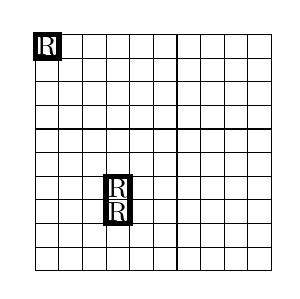
\begin{tikzpicture}[scale=0.3]
		\draw (0,0) -- (10,0) -- (10,10) -- (0,10) -- cycle;
		\draw (0,1) -- (10,1);
		\draw (0,2) -- (10,2);
		\draw (0,3) -- (10,3);
		\draw (0,4) -- (10,4);
		\draw (0,5) -- (10,5);
		\draw (0,6) -- (10,6);
		\draw (0,7) -- (10,7);
		\draw (0,8) -- (10,8);
		\draw (0,9) -- (10,9);


		\draw (1,0) -- (1,10);
		\draw (2,0) -- (2,10);
		\draw (3,0) -- (3,10);
		\draw (4,0) -- (4,10);
		\draw (5,0) -- (5,10);
		\draw (6,0) -- (6,10);
		\draw (7,0) -- (7,10);
		\draw (8,0) -- (8,10);
		\draw (9,0) -- (9,10);
		\draw (10,0) -- (10,10);

		\node at (0.5,9.5) {R};
		\node at (3.5,2.5) {R};
		\node at (3.5,3.5) {R};
		\draw[line width=2pt] (3,2) -- (4,2) -- (4,4) -- (3,4) -- cycle;
		\draw[line width=2pt] (0,9) -- (0,10) -- (1,10) -- (1,9) -- cycle;
	\end{tikzpicture}
\end{center}

\noindent
Jeśli pole nie zawiera rośliny, a co najmniej dwa sąsiednie pola ją zawierają, to co najmniej dwa boki tego pola są dzielące. Stąd też, jeśli w tym polu wyrośnie roślina, to łączna długość krawędzi dzielących się nie zwiększy.

\vspace{10px}
\noindent
Początkowo łączna długość krawędzi dzielących wynosi co najwyżej $4 \cdot 9 = 36$. Jeśli roślina porosłaby całą planszę, to dzielące byłby wszystkie krawędzie leżące na boku dużego kwadratu. Ich długość wynosi $40$. Skoro więc ta liczba nie zwiększa się, to nigdy stan, w którym wyniesie ona $40$, nie zostanie uzyskany.

\vspace{5px}

\begin{problem}{5}
	Każdy punkt płaszczyzny pokolorowano jednym z dwóch kolorów. Wykazać, że istnieje taki trójkąt o kątach $80\degree$, $80\degree$ i $20\degree$, że wszystkie jego wierzchołki są jednego koloru.
\end{problem}

\noindent
Oznaczmy kolory numerami $1$ i $2$.
Najpierw wykażemy, że istnieją takie punkty $A$, $B$, że są one jednakowego koloru oraz środek odcinka $AB$ jest tego samego koloru co one.
Rozpatrzmy dowolne dwa punkty na płaszczyźnie, które są tego samego koloru. Nazwijmy je $X_1$ i $X_2$ oraz przyjmijmy, że są koloru $1$. Niech punkty $Y_1$ i $Y_2$ leżą na prostej $X_1X_2$, tak, że punkty $X_1$, $X_2$ są środkami odpowiednio odcinków $Y_1X_2$ i $Y_2X_1$. Zauważmy, że odcinki $X_1X_2$ oraz $Y_1Y_2$ mają wspólny środek -- nazwijmy go $M$.

\begin{center}
	\begin{tikzpicture}[]
		\tkzDefPoint[label = above:$Y_1$](0,0){Y_1}
		\tkzDefPoint[label = above:$X_1$](2,0){X_1}
		\tkzDefPoint[label = above:$M$](3,0){M}
		\tkzDefPoint[label = above:$X_2$](4,0){X_2}
		\tkzDefPoint[label = above:$Y_2$](6,0){Y_2}

		\tkzDrawPoints(X_1, Y_1, X_2, Y_2, M)
		\tkzDrawSegments(Y_1,Y_2)
	\end{tikzpicture}
\end{center}

\noindent
Jeśli $Y_1$ jest koloru $1$, to trójka jednokolorowych punktów $Y_1$, $X_1$ i $X_2$ tworzy odcinek ze środkiem. Rozpatrzmy więc przypadek, gdy $Y_1$ jest koloru $2$. Analogicznie rozumując dochodzimy do wniosku, że $Y_2$ jest koloru $2$.

\vspace{10px}
\noindent
Jeśli $M$ jest koloru $1$, to trójka $X_1$, $M$ i $X_2$ spełnia warunki zadania. Gdy zaś $M$ jest koloru $2$, to trójka $Y_1$, $M$ i $Y_2$ spełnia warunki zadania.

\vspace{10px}
\noindent
Rozpatrzmy trójkąt $ABC$ o kątach danych w treści, w którym środki boków $AB$, $BC$ i $CA$ oznaczamy jako $N$, $S_1$ i $S_2$. Na mocy tego, co pokazaliśmy powyżej, można wybrać taki trójkąt, że $A$, $N$ oraz $B$ będą jednego koloru -- powiedzmy, że będzie to kolor $1$.

\begin{center}
	\begin{tikzpicture}[]
		\tkzDefPoint[label = below:$A(1)$](0,0){A}
		\tkzDefPoint[label = below:$B(1)$](4,0){B}
		\tkzDefPoint[label = above:$C$](3.76,1.37){C}
		\tkzDefMidPoint(A,B) \tkzGetPoint{N}
		\tkzDefMidPoint(B,C) \tkzGetPoint{S_1}
		\tkzDefMidPoint(C,A) \tkzGetPoint{S_2}

		\tkzLabelPoint[below](N){$N(1)$}
		\tkzLabelPoint[above right](S_1){$S_1$}
		\tkzLabelPoint[above left](S_2){$S_2$}

		\tkzDrawPoints(A,B,C,N,S_1,S_2)
		\tkzDrawSegments(A,B B,C C,A)
	\end{tikzpicture}
\end{center}

\noindent
Zauważmy, że jeśli jakikolwiek z punktów $C$, $S_1$ i $S_2$ byłby koloru $1$, to wówczas jeden z trójkątów $ABC$, $ANS_2$, $ABS_1$ byłby jednokolorowy. Jeśli zaś wszystkie punkty $C$, $S_1$ i $S_2$ są koloru $2$, to one same tworzą trójkąt jednokolorowy.
\vspace{5px}

\begin{problem}{6}
	Prostokąt $\mathcal{P}$ o wymiarach $1001 \times 1001$, podzielono na pewną liczbę prostokątów, z których każdy ma boki długości całkowitej (przykład na rysunku). Wykazać, że z tych prostokątów można wybrać taki jeden, że odległości jego czterech boków od odpowiadających mu boków $\mathcal{P}$ albo są wszystkie liczbami parzystymi, albo są wszystkie liczbami nieparzystymi.

	\begin{center}
	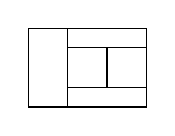
\begin{tikzpicture}[scale=0.5]
		\draw (0,0) -- (3,0) -- (3,2) -- (0,2) -- cycle;
		\draw (0,0) -- (1,0) -- (1,2) -- (0,2) -- cycle;
		\draw (1,0) -- (3,0) -- (3,0.5) -- (1,0.5) -- cycle;
		\draw (1,1.5) -- (3,1.5) -- (3,2) -- (1,2) -- cycle;
		\draw (2,0.5) -- (3,0.5) -- (3,1.5) -- (2,1.5) -- cycle;
	\end{tikzpicture}
\end{center}
\end{problem}

\noindent
Pokolorujmy ten prostokąt w szachownicę. Załóżmy, że lewe dolne pole będzie koloru czarnego. Skoro prostokąt $\mathcal{P}$ ma bok nieparzystej długości, to wszystkie jego narożne pola będą koloru czarnego. Również zawiera on o jedno pole czarne więcej niż zawiera pól białych. 

\vspace{10px}
\noindent
Każdy z prostokątów, na które jest on podzielony można zaklasyfikować do jednego z trzech typów:
\begin{itemize}
	\item Prostokąt, który ma dwa pola narożne białe i dwa pola narożne czarne. Zawiera on tyle samo pól białych, co czarnych;
	\item Prostokąt o czterech polach narożnych białch. Zawiera on o jedno pole białe więcej;
	\item Prostokąt o czterech polach narożnych czarnych. Zawiera on o jedno pole czarne więcej.
\end{itemize}

\begin{center}
	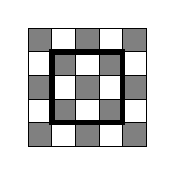
\begin{tikzpicture}[scale=0.3]

		\fill[color=gray] (0,0) rectangle (1,1);
		\fill[color=gray] (1,1) rectangle (2,2);
		\fill[color=gray] (2,2) rectangle (3,3);
		\fill[color=gray] (3,3) rectangle (4,4);
		\fill[color=gray] (4,4) rectangle (5,5);
		\fill[color=gray] (0,4) rectangle (1,5);
		\fill[color=gray] (0,2) rectangle (1,3);
		\fill[color=gray] (1,3) rectangle (2,4);
		\fill[color=gray] (2,4) rectangle (3,5);
		\fill[color=gray] (2,0) rectangle (3,1);
		\fill[color=gray] (3,1) rectangle (4,2);
		\fill[color=gray] (4,2) rectangle (5,3);
		\fill[color=gray] (4,0) rectangle (5,1);

		\draw (0,0) -- (5,0) -- (5,5) -- (0,5) -- cycle;
		\draw (0,1) -- (5,1);
		\draw (0,2) -- (5,2);
		\draw (0,3) -- (5,3);
		\draw (0,4) -- (5,4);


		\draw (1,0) -- (1,5);
		\draw (2,0) -- (2,5);
		\draw (3,0) -- (3,5);
		\draw (4,0) -- (4,5);

		\draw[line width=2pt] (1,1) rectangle (4,4);
		
	\end{tikzpicture}
\end{center}

\noindent
Skoro $\mathcal{P}$  zawiera o jedno pole czarne więcej, to pewien z rozpatrywanych prostokątów, nazwijmy go $P$ musi mieć czarne pola narożne. Zarówno $\mathcal{P}$, jak  $P$ mają czarne pola narożne, z czego łatwo wynika, że odległości między odpowiadającymi im bokami są tej samej parzystości.